\documentclass[11pt]{article}

\usepackage[margin=1in]{geometry}
\usepackage[T1]{fontenc}
\usepackage{amsmath,amssymb}
\usepackage{booktabs,array}
\usepackage{graphicx}
\usepackage{xcolor}
\usepackage[numbers,sort&compress]{natbib}
\PassOptionsToPackage{hyphens}{url}
\usepackage[colorlinks=true,linkcolor=blue!50!black,citecolor=blue!50!black,urlcolor=blue!50!black]{hyperref}

\newcommand{\cmd}[1]{\texttt{#1}}
\setlength{\emergencystretch}{2em}
\newcommand{\um}{\,$\mu$m}
\newcommand{\degC}{\,$^\circ$C}

\title{Translucent: an agent that turns recorded battery experiments\\into checked findings and sealed intervention decisions}
\author{Translucent team}
\date{Draft of 30 October 2026}

\begin{document}
\maketitle

\begin{abstract}
Laboratories hold far more recorded observations than they can analyse: microscope movies, thermocouple traces,
voltage logs and the tables of published papers. An agent with vision models can read these records, but it can
also turn a wrong clock or a copied number into a confident finding. We describe Translucent, an agent that reads
recorded experiments with Meta's models (Muse Wonder plans, Muse Spark reads frames and tables, SAM~3.1 outlines
objects) and turns them into findings and decisions whose every number traces to a recorded measurement. Fixed code, not a model,
decides which findings are supported; every record is kept in an insert-only ledger that a single command re-checks
offline. We report two demonstrations. First, on published dendrite and graphite-plating movies, the deterministic
checks caught 24 of 24 planted data mistakes (38 of 38 planted faults in all) against 1 for a plain analysis
pipeline, including a playback clock that makes filaments appear to grow 18 times faster than they did; a model
reviewer given only a finding and its numbers let 5 of 18 planted mistakes through, and caught all 18 when given the
full evidence record. Second, we extend the loop from findings to actions on NIST's 2026 heat-interruption trials of
18650 and 21700 cells: at heater-off the agent must stand down, escalate, or watch 30 or 60~s more, and it commits
each decision and its probability before the sealed recorded outcome is revealed. The protocol, splits, baselines
and decision rule were fixed before held-out scoring, after two disclosed amendments. On the registered primary
analysis (leave one condition out, 50 trials) neither of the agent's learning strategies beats always escalating
after correction: mean decision cost 3.72 and 3.80 per trial against 3.80 (Holm-corrected $p = 1$). Its three
registered wins come from a difference in decision rules and from physics baselines that do not discriminate, not
from anything the agent learned, and none survives a test that respects condition clustering. The contribution of
the second demonstration is therefore the loop itself, in which every forecast, decision and score can be
recomputed offline and any edit to the record is detected, and the negative result, which we report as a finding.
Live campaigns in which Muse Wonder chooses the strategies reach the same result (best 3.00 and 3.40 against 3.80,
Holm $p = 1$), and the gate refused the planner's own claim that its policy beat always escalating.
\end{abstract}

% ======================================================================================================== 1
\section{Introduction}\label{sec:intro}

Battery laboratories record more than they analyse. A single operando microscopy study produces movies with their
own clocks and scale bars, a voltage log, and a paper whose figures and tables summarise them. A thermal-abuse study
produces hundreds of thermocouple traces, a few edited videos, and tables whose cell colours carry the outcomes. Vision
and language models can now read all of these records. The difficulty is not reading them but keeping what is read
honest. In one published movie that we use below, each captured image is 6.9~s of lab time but 0.4~s of playback;
an analysis that times the playback reports filaments growing 18.2 times faster than they did, and nothing in the
output warns about it. An agent that plans tests and writes analysis code can carry such an error into a finding
and then into a decision.

The decisions we care about here are actions on a physical system under hidden state. From US national fire-incident
and consumer-product records, NIST estimates about 198{,}000 lithium-ion battery fires in structures since 2011 (95\%
CI 84{,}000--465{,}000), with consumer battery fires growing by about 10\% per year (CI 7.1--13.0\%)
\citep{gilbert2026risk}. For grid-scale storage,
EPRI reports a large fall in failures per deployed GWh between 2018 and 2025, and cautions against using the rate for
prediction \citep{epri2026bess}. NIST's 2026 heat-interruption study asks a concrete question about these commercial
cells: once an externally heated cell has vented, can cutting the heat still prevent ignition, and for how long
\citep{tam2026intervention}? These statistics and that study concern commercial 18650 and 21700 cells. The dendrite
and plating movies of Section~\ref{sec:demo1} concern laboratory solid-state and graphite cells, a different physical
system; we do not transfer any result between them.

\paragraph{Thesis.} Existing experimental observations, including unstructured visual evidence, can be turned into
executable, uncertainty-aware decisions about what to do to a physical system, without each laboratory building its
own agent stack, provided that (i) every number the agent reports is a recorded measurement with recorded provenance,
(ii) fixed code rather than a model decides what is supported, (iii) a decision about an action is committed before
its outcome is revealed, and (iv) the system updates only after measured feedback, through a deterministic gate, in a
record anyone can re-check offline. The loop is: observe (Muse Spark and SAM~3.1); state competing mechanistic
hypotheses (Muse Wonder); build executable world models whose action-conditioned forecasts are labelled simulated;
commit a bounded intervention decision before the outcome is revealed; score it on the real recorded outcome; and
update only after that feedback (Figure~\ref{fig:loop}).

\begin{figure}[t]
  \centering
  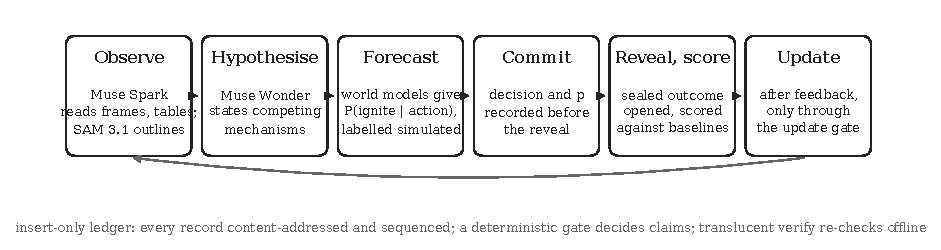
\includegraphics[width=\linewidth]{figures/fig_loop.pdf}
  \caption{The loop. Observation and hypotheses come from Meta's models; forecasts come from executable world models
  and are labelled simulated; the decision is recorded before the sealed outcome is opened; updates pass a
  deterministic gate. Every step writes to the same insert-only ledger.}
  \label{fig:loop}
\end{figure}

\paragraph{Contributions.}
\begin{enumerate}
  \item A harness for agents on recorded experiments: an insert-only evidence ledger, a deterministic claim gate, a
  perturbation check that rejects numbers typed into agent-written analysis code, recorded and replayed model calls,
  and an offline verifier that re-derives every verdict from the ledger as it stood when the verdict was recorded
  (Section~\ref{sec:system}).
  \item A measured demonstration on observation (Section~\ref{sec:demo1}): planted-mistake results against a plain
  pipeline and against a model reviewer, agreement with published timings, a team campaign with people in the loop,
  and the failures we found in our own agent.
  \item A factual intervention benchmark built on NIST's heat-interruption data, with its data traps documented,
  outcomes sealed and committed-before-revealed, a protocol and decision rule fixed before held-out scoring, nine
  registered baselines, and an offline verifier that refits every model and re-derives every scored decision
  (Section~\ref{sec:demo2}).
  \item A record of negative and limiting results: a model reviewer that waves mistakes through without the evidence
  record, a visual second opinion that disagrees with correct findings, a memory mechanism that slowed the agent,
  lumped physics that cannot forecast ignition from pre-decision data, no transfer across cell format, learned
  intervention policies that do not beat always escalating, and an earlier version of our own verifier that accepted
  four kinds of forged record.
\end{enumerate}

% ======================================================================================================== 2
\section{Related work}\label{sec:related}

\paragraph{Agents that drive instruments.} Argonne connected an agent to Meta's SAM~3 to turn plain-language requests
into self-guided experiments at a hard X-ray nanoprobe, and is making SAM~3 available across DOE facilities
\citep{argonne2026synaps}. DOE's 2026 robotics and automation selections ask for digital twins, benchmark tasks,
safety practices and provenance records \citep{doe2026robotics}. Qiushi ran an end-to-end discovery study on a real
optical platform with 3{,}242 model calls and 1{,}242 tool calls \citep{yang2026qiushi}; we found no public code or
data for it. Robin, a multi-agent system, proposed a therapeutic candidate for dry age-related macular degeneration
that human researchers then tested in cell assays \citep{ghareeb2026robin}, and Lila's human-supervised platform
evaluated 2{,}942 catalysts across 53 material systems \citep{jenewein2026lila}. Autonomous scanning electrochemical
cell microscopy predicted a composition-activity trend after measuring 15\% of 966 areas, and because every area was
measured, the choice of the next measurement can be scored against measured ground truth \citep{thelen2026seccm}.
These systems act on instruments. Translucent does not control an instrument; it works on recordings, and its
emphasis is on what a recorded number may be used to claim, and on committing decisions before outcomes are seen.

\paragraph{World models and interventions.} Asking the World builds an executable world from video and then queries,
simulates and intervenes on it \citep{zeng2026asking}. RSI-Anything uses predictive world models to guide action and
data selection; observed feedback drives policy improvement and \emph{conditional} world-model adaptation, and
component and compatibility checks govern whether an updated policy-model pair is kept \citep{cui2026rsianything}.
AbsorbEvo has one language model propose design changes for microwave absorbers, ranks them with a low-cost
predictive model, and sends only high-ranking designs to full-wave simulation, reaching 79.17\% task success against
25.00\% for a generic agent and 12.50\% for random search on held-out tasks \citep{feng2026absorbevo}. We share the
executable world model with the first, the update-only-after-feedback compatibility gate with the second, and the
cheap-screen-then-expensive-test funnel with the third. We differ in three ways: our forecasts are labelled simulated
and can never alone support a claim; every outcome we score is a recorded physical outcome, not a simulation; and the
number of candidates the agent sends to the expensive test is counted from the ledger and used in a multiple-comparison
correction.

\paragraph{Prediction is not mechanism.} CausaLab shows a gap between prediction and mechanism recovery: in a purely
observational six-node setting a frontier model reaches 92\% task accuracy but 0.471 all-edge F1, and mixing
observation with intervention improves structural fidelity \citep{yang2026causalab}. What-If World finds that none
of the nine general world models it tested exceeds 52\% on paired counterfactual prompts \citep{cai2026whatif}. Both motivate two choices
here: we never present an unobserved counterfactual as observed, and we rank proposed next experiments by how
strongly competing hypotheses disagree about their outcome, not by outcome uncertainty alone.

\paragraph{Closed loops on batteries.} Attia et al.\ optimised fast-charging protocols in closed loop over 224
candidates \citep{attia2020closed}, building on early cycle-life prediction \citep{severson2019data}. The closed-loop
rounds ran 100 cycles, so most protocol outcomes are early predictions; nine protocols were tested to failure with
five cells each. In the released validation file the top five protocols lie within 42 cycles of each other with 95\%
intervals of $\pm$78 to $\pm$148 cycles, so a pick-the-best benchmark on them separates about three tiers. Our task is
different: one safety action per trial, scored on its recorded outcome, with the decision sealed before the reveal.

\paragraph{Why not the Stanford compression study.} Cui et al.\ show that biaxial compression of a solid electrolyte
deflects dendrites and prevents short-circuiting at 100~mA\,cm$^{-2}$ \citep{cui2026dendrite}. It is the most direct
recent example of an intervention against dendrite shorting, and its data are open \citep{cui2026dendrite_data}. We
did not build on it: the archive is figure source data for one stress level and a handful of cells (one stressed and
one unstressed cell per figure), with no sweep over the intervention and no trials that could be held out. It could
support a worked example, not a scored benchmark.

% ======================================================================================================== 3
\section{System}\label{sec:system}

Translucent runs a campaign: a research question, the recorded experiments it concerns, a budget, and a planner
model that calls tools. Tools read the recordings and write measurements; the planner proposes findings; a gate
decides them. This section describes the parts that make a result checkable. Code paths are given relative to the
repository root.

\subsection{The ledger}
The ledger (\cmd{translucent/ledger.py}) is a SQLite database plus a content-addressed file store. Every file is
stored under its SHA-256 and recorded as an artifact; re-adding identical bytes returns the existing record. Records
are typed (campaign, artifact, run, measurement, claim, review, lesson, fork, protocol, decision) and stored as JSON
in one table. Database triggers abort every \texttt{UPDATE} and \texttt{DELETE} on records, events and
invalidations, so a change of status is always a new row: a review for a claim, an invalidation for a run. Derived
state is computed from history, never stored. A claim's status is the latest gate verdict, or \emph{stale} if any
measurement it cites, or anything that measurement was derived from, came from a run invalidated later.

Admission rules run on insert. A measurement must cite an existing run whose status is \emph{ok} and which lists it
among its outputs; its calibrations and source artifacts must exist; an artifact made only by failed runs cannot back
a measurement. A claim must cite existing measurements. A protocol is admitted only before its campaign has started
or recorded any work. Events receive a per-campaign sequence number assigned inside the insert transaction, so the
order in which things happened is part of the record.

\subsection{The gate}
The gate (\cmd{translucent/gate.py}) is deterministic code with no model call. It returns one of four verdicts:
\emph{supported}, \emph{refuted}, \emph{inconclusive}, or \emph{unsupported}. Unsupported means the evidence cannot
carry the claim and says nothing about the science; a tool failure or a malformed finding can never produce
\emph{refuted}. Before any arithmetic it checks provenance for every cited measurement: the producing run succeeded
and has not been invalidated; the measurement traces to a recorded video; a physical unit has the calibrations it
needs (a length needs a spatial scale, a time or rate needs a time base), those calibrations come from the
experiment's own records rather than from agent output, and they belong to the same recording; no other trusted scale
for that recording disagrees beyond both uncertainties; and a finding that needs independent corroboration has it
(a short-circuit time must be accompanied by the instrument's recorded voltage-collapse time).

Four predicate types are evaluated from the cited measurements and their stated uncertainty, converted to a
half-width $h$ (twice the standard deviation for a standard error, the stated value for a bound or interval).
\texttt{value\_within} is supported if $[v-h, v+h]$ lies inside the claimed range, refuted if the two are disjoint,
and inconclusive otherwise; a range wider than half the magnitude of its ends is inconclusive by rule, because a
test that loose cannot tell values apart. \texttt{values\_agree} and \texttt{events\_coincide} compare
$|a-b|$ with $t + \sqrt{h_a^2+h_b^2}$ for a stated tolerance $t$, and \texttt{trend} fits a least-squares slope with
a two-standard-error interval. The agent writes the finding's sentence; the gate's recorded checks state the numbers
it actually tested.

\subsection{Agent-written analysis and the perturbation check}
The planner may write Python analysis code (\cmd{translucent/analysis.py}). It runs in a fresh, network-blocked
sandbox that receives only the ledger records the planner names as inputs and must write exactly the declared outputs,
each a finite number with an optional uncertainty. The code is stored as an artifact, and each output is recorded as a
\texttt{derived:} measurement that inherits the calibrations and sources of its inputs.

A model can satisfy every structural rule and still type numbers into the code. We found that our own planner did
this (Section~\ref{sec:typed}). The check that followed runs the same code a second time on its recorded inputs with
every number moved by 0.2--0.5\%, with an independent random sign per number drawn from an unpredictable seed. An
output, or a stated uncertainty, that does not move (relative tolerance $10^{-6}$) is rejected with the reason, and
the run fails. Code that reads no recorded measurement is rejected outright.

\subsection{Recorded model calls}
SAM~3.1 is non-deterministic and paid, so every live response is stored once, keyed by a hash of the media content,
prompt and settings (\cmd{translucent/recordings.py}). In the default strict mode, replay serves only an exact match
and otherwise fails; it never re-calls the service or substitutes a near match. Because remuxed and decoded video
bytes differ between FFmpeg builds, a recording also carries a hash of the video's encoded packets, and replay falls
back to the same source with the same prompt and settings. A development-only mode that serves the nearest recorded
frame records the substitution in the tool run. All paid calls are metered against hard provider caps. Campaign
events record each planner step, tool run and cost, so a finished campaign can be browsed, replayed and verified
without provider keys; the offline evaluations run tools against the recorded SAM outputs.

\subsection{Receipts and offline verification}
\cmd{translucent verify} (\cmd{translucent/verify.py}) accepts a ledger or an exported bundle and exits 0 only if
everything matches. It works on a snapshot copy. It checks database integrity and that the insert-only triggers are
present and unchanged; every file's bytes against its content address and recorded size; that event sequences have no
gaps and clocks never run backwards; and that every recorded measurement and tool completion matches its event. It
then re-runs the gate for every recorded gate review on the ledger \emph{as it stood when that review was recorded}:
inside a savepoint it removes every row inserted at or after the review and every later invalidation, re-runs the
gate, compares verdict, checks and reason, and rolls back. For supported findings it walks the full evidence graph
(measurements, runs, inputs, artifacts and their parents) and reports any failed or invalidated ancestor. It also
re-checks what-if branches, that each protocol preceded its campaign's start, and every recorded method decision.
An exported bundle carries a manifest of file hashes and a ledger snapshot holding only the records the campaign
needs; verification compares the bundle's campaign, events, findings, reviews and records with that snapshot.

For intervention campaigns (Section~\ref{sec:demo2}) verification goes further, because there a controller rather
than the gate produces most records. It rebuilds every fitted model from exactly the revealed training trials
registered for its fold and compares it with the stored one; recomputes every screen and its survivors; re-derives
every committed decision from its stored model, decision rule and the observations the policy paid for; checks that
every scored decision precedes its trial's reveal and that every reveal matches its seal; checks each paid watch trace
against the revealed ignition time; requires every model-made decision to be bound to exactly one earlier recorded
model request and response; and recomputes every score, paired test and Holm correction. These checks were added after
an independent code review of an earlier version, which reproduced four forged ledgers that verification accepted: a
model fitted on held-out labels, Muse-only decisions with no provider receipts, an edited ignition time and censoring
flag, and twelve ignition times moved past the watch window, which turned 12 unsafe watches into none. Each now fails
verification with a specific reason (for example, a stored threshold of 161.275 against a refit of 161.3025, or a paid
observation that contains an ignition jump at 520~s when the revealed ignition time is 995~s), while an honest control
ledger still verifies. The full test suite passes (799 tests, 1 skipped). We report this as a strength of the process: the
verifier is itself tested against forgeries, and it was strengthened when a review found a gap.

\subsection{People in the loop}
People act through an authenticated HTTP API. A note reaches the planner before its next step. The planner can ask a
person a question (for example, which cell this is, or how long the scale bar is) and waits a bounded time before
carrying on with the records it has. People can pause or stop a campaign. A sign-off or a challenge is recorded as a
review with \texttt{reviewer = human} and the person's name; it never changes a claim's status, which only the gate
decides. A challenge is passed to the planner for re-examination. Each sign-off is shown with a digest of the
evidence the person reviewed, so a later invalidation is visible as ``evidence changed since this review''. Text from
people, experiment manifests and agent-written code is scrubbed of secret-looking strings before it is recorded, and
people's writes accept an idempotency key.

\subsection{Pre-registered metrics and method decisions}
A protocol (\cmd{translucent/protocol.py}) fixes, before a campaign starts, which quantities count for each metric,
the unit, and the exact gate test. A finding is \emph{on protocol} only if its test is exactly the metric's; others
are still checked but can never win. Declaring a winning method requires the minimum number of distinct methods
(tool and code hash), a supported on-protocol winner, a supported verification finding that re-derives the winner's
value through runs it shares with nothing but the experiment's own records, every replication succeeded, and no
supported on-protocol attempt by another method disagreeing. The verifier re-derives every recorded decision on the
ledger as it stood.

\subsection{Models and roles}
Table~\ref{tab:models} lists the roles. The \texttt{meta} profile used in the campaigns of
Section~\ref{sec:demo1} runs the planner on Muse Wonder (\texttt{muse-wonder-1.0}) and the frame reader on Muse Spark
(\texttt{muse-spark-1.3}) through the Meta Model API \citep{meta2026modelsdocs}; SAM~3.1 runs through the same API
\citep{meta2026segmentation}; the advisory second opinion runs on Muse Spark Open served by Fireworks. A
\texttt{dev} profile runs every role on Muse Spark Open and replays recorded SAM calls.

\begin{table}[t]
\centering\small
\caption{Model roles. Every role that reads or writes evidence goes through the ledger; none decides a verdict.}
\label{tab:models}
\begin{tabular}{@{}p{3.0cm}p{3.6cm}p{8.4cm}@{}}
\toprule
Role & Model & What it does \\
\midrule
Planner & Muse Wonder & Chooses tests, writes analysis code, reads rejection reasons, asks people for missing facts; in Section~\ref{sec:demo2}, states hypotheses and proposes policies \\
Reader (pointer) & Muse Spark & Returns pixel points on a gridded frame; reads table images and burned-in video overlays \\
Outliner & SAM~3.1 & Converts points and boxes to masks; segments the ignition jet in the NIST videos; every call recorded \\
Second opinion & Muse Spark Open & Reviews one evidence image after a finding is supported; advisory only \\
Gate, verifier & none (fixed code) & Decides findings and re-checks them offline \\
\bottomrule
\end{tabular}
\end{table}

% ======================================================================================================== 4
\section{Demonstration 1: observation with receipts}\label{sec:demo1}

\paragraph{Data.} We use the supplementary movies of two open-access papers: Movies~1 and~4 of Reisecker et al., which
film lithium filaments growing through a solid electrolyte under pulsed current \citep{reisecker2023dendrite}, and
Movie~1 and the source data of Lu et al., which film graphite during fast charging \citep{lu2023graphite}. Both are
CC~BY~4.0. The published numbers we compare against are digitised with provenance in \cmd{data/groundtruth/}.

\subsection{Planted mistakes}
The fault-injection suite (\cmd{evals/run.py}, results \cmd{evals/results/20261029T161733.json}, report
\cmd{evals/REPORT.md}) builds a fresh ledger for each case, plants one fault, runs the real tools or inserts the faulty
record, and then proposes the \emph{naive} finding, which is exactly what the faulty evidence shows. Only a check that
notices the fault can stop it; a number that happens to disagree cannot. The plain pipeline baseline
(\cmd{evals/baseline.py}) takes SAM's boxes, converts pixels with whatever scale it is given, times every playback
frame at the file's frame rate, fits a line and reports the number; it catches a fault only if it crashes or outputs
a non-finite value. The suite ran offline with replayed SAM calls and network sockets disabled.

\begin{table}[t]
\centering\small
\caption{Planted faults caught (the faulty evidence did not become a supported finding). The first five classes are
faults a plain script also faces; the last three concern the evidence record itself and have no analogue in a plain
script.}
\label{tab:faults}
\begin{tabular}{@{}lrrr@{}}
\toprule
Fault class & Cases & Translucent & Plain pipeline \\
\midrule
Spatial calibration (wrong, foreign or missing scale) & 5 & 5 & 1 \\
Time base (playback frames used as lab time) & 4 & 4 & 0 \\
Swapped video & 3 & 3 & 0 \\
Junk masks (whole-sample, merged or low-confidence outlines) & 9 & 9 & 0 \\
Missing corroboration & 3 & 3 & 0 \\
\midrule
\emph{Data-path subtotal} & 24 & \textbf{24} & 1 \\
\midrule
Fabricated measurement (including numbers typed into code) & 8 & 8 & 0 \\
Retracted evidence & 3 & 3 & 0 \\
Second-opinion overreach & 3 & 3 & 0 \\
\midrule
\emph{All faults} & 38 & \textbf{38} & 1 \\
\bottomrule
\end{tabular}
\end{table}

Table~\ref{tab:faults} gives the result. The plain pipeline's one catch was a length with no scale, which raised a
type error. Across the 38 cases, Translucent stopped the fault through a gate verdict (11 unsupported, 2 refuted), a
tool refusal such as a scale from another experiment or a video imported under the wrong experiment (6), an
outline-quality flag (8), an admission rule (7), staleness after invalidation (3), or, for a second-opinion review of
a claim the gate never saw, by leaving the claim at \emph{proposed} (1). Two weak spots remain on record in the
report: without a recorded clock, repeated playback frames are not collapsed into captured images (the gate still
refuses the resulting speed), and the second opinion runs only after the gate says supported, so a fault the gate
missed would reach it with nothing else behind it.

\subsection{The 18-fold clock error and agreement with the paper}
A scripted filament grows 1~px per recorded second on Movie~4's real clock and scale; the truth is 6.203\um/s.
Translucent measures $6.200 \pm 0.018$\um/s (95\% interval) and the gate supports a claim within 10\% of the truth.
The plain pipeline, timing playback frames, reports $112.82$\um/s, 18.2 times too fast. On Movie~1, which has no
recorded clock, both report $741.75 \pm 91.07$\um\ per playback second; Translucent refuses to support it as a speed.

On Movie~4's real voltage log, the first short is measured at $89.55 \pm 3.45$~s, recovery at $214.95 \pm 3.45$~s and
the second short at $351.3 \pm 6.7$~s (bounds). The paper's voltage data place these at 86--93~s, 211--218~s and
345--358~s; each measured window overlaps the published one.

\subsection{A team campaign with people in the loop}
The Movie~4 team campaign (\cmd{web/public/fixtures/m4-team/}) ran live on Meta's models over the HTTP API. Muse
Wonder planned, Muse Spark located filament lanes, and SAM~3.1 outlined them. Before the first step a scientist (Ana)
left a note describing the electrodes and the five lanes where filaments grow; the agent outlined those lanes. The
agent proposed 12 findings; the gate supported 7, judged 4 inconclusive and 1 unsupported. The supported findings
include the first short ($89.55 \pm 3.45$~s), recovery ($214.95 \pm 3.45$~s), the second short ($351.3 \pm 6.7$~s),
an initial growth speed of 55--72\um/s ($63.7 \pm 4.0$, standard error of the fitted slope), retraction at 48--73\um/s, and a typical
filament length near 1439\um\ ($\pm 38$, standard error). Ana signed off the first short. A second scientist (Ben) challenged the
growth speed, asking whether it came from the growing phase only, before the first short; the agent recomputed it
from points before the short and the gate supported that narrower finding. The campaign did not prove that a filament
bridged the electrode gap, and recorded a lesson: an outline measured from one electrode can merge with the far
electrode, so the tip must be checked against both edges. \cmd{translucent verify} re-checks 12 of 12 findings
offline. Metered model spend was \$3.00 (planner \$2.72, reader \$0.25, second opinion \$0.04).

\subsection{The agent typed numbers in}\label{sec:typed}
The first Meta-model run on Movie~4 also ``proved'' a growth speed, a filament length and an electrode gap. Reading
the evidence showed that the planner's sandboxed code had copied numbers from earlier tool output and chosen its own
error bars; it had not read the recorded measurements it declared as inputs. The gate could not see this, because
the code's declared inputs were valid. This failure led to the perturbation check of Section~\ref{sec:system}, and it
is now a planted case in Table~\ref{tab:faults}. The earlier run is kept as evidence of the failure
(\cmd{web/public/fixtures/m4-meta/}); both demonstration campaigns were re-run with the check in place, and every
analysis number in them passed it.

\subsection{Graphite during fast charging}
On Lu et al.'s graphite movie (\cmd{web/public/fixtures/lu-live/}), the gate supported that cell voltage first fell
below 0~V after $7.435 \pm 0.68$~h of charging, $2.565 \pm 0.68$~h before the paper's stated plating onset of 10~h.
Under the assumptions that the stated onset means the first 0~V crossing and that the voltage error is within
$\pm$10~mV, the two cannot be reconciled; we do not claim the paper is wrong. The campaign did not prove a visual
plating onset: no silver-grey layer distinct from the gold colour of lithiated graphite was bracketed between a last
clean and a first coated frame, and the movie clock bound of about $\pm$20 minutes is too coarse. It recorded a lesson
that the gold lithiation colour can be mistaken for plating. Metered spend was \$0.88.

\subsection{What a model reviewer sees}
Could a model replace the gate? We asked Muse Spark Open to judge every finding the planted mistakes produced, three
times each (\cmd{evals/llm\_judge.py}; \cmd{evals/LLM\_JUDGE.md}; 120 calls, \$0.95). Twenty of the 38 cases were
stopped before any finding existed, leaving 18 judged planted mistakes and two correct controls. Given a finding and
its numbers, the model accepted 5 of 18 planted mistakes (4 of 11 data-path mistakes) and rejected 1 of 2 correct
findings. Given the full evidence record as text (measurements, competing calibrations, runs, inputs, artifact
ancestry, sources, clock sources and invalidations), it caught all 18 and accepted both correct findings. The
evidence given to a reviewer decides the result. The gate checks that record for every finding without a model call.

\subsection{Limits of the visual second opinion}
After the gate supports a finding, a vision model reviews one evidence image: the voltage log with the finding's
times marked, or a frame. In 16 seeded cases run three times each (48 calls, \$0.21;
\cmd{evals/results/critic-real-20261028.json}), it never agreed with a wrong or unreadable finding (0 of 33) and missed
a correct finding in 3 of 15 runs (20\%), all three on the same correct first-short case. In the live campaigns it
reviewed 9 supported findings: it agreed with 4, was inconclusive on 3 and disagreed with 2 (the second short and the
typical length in the team campaign), although the gate's second-short window overlaps the paper's. Its verdicts are
recorded beside the gate's and change nothing.

\subsection{A weak spot in memory}
Lessons are recorded with their evidence and loaded at the next campaign's start. In a real test (Muse Spark Open for
every role, three repeats per arm, \$0.37; \cmd{evals/MEMORY.md}), a lesson about filament bridging led the agent
into unnecessary video analysis for a question about short timing: 11.3 steps on average with the lesson against 6.3
without, with the same 3 findings. At the time every lesson in the ledger was loaded whatever the question. Loading
has since been restricted to at most six lessons that concern the same recording, the same source, or a method in
general, with confidence derived from the record (\cmd{translucent/memory.py}); that change has not been re-measured,
and $n=3$ per arm is a direction, not a statistical result.

\subsection{Observations on the models}
SAM~3.1 text prompts such as ``dendrite'' or ``thin dark line'' returned no masks on these microscopy frames; point
and box prompts worked, so Muse Spark supplies points for SAM to outline. On Movie~1 SAM's filament tip agreed with a
classical tip detector to a median of 4.5~px. Video tracking worked forward only, and rapid growth between captured
images in Movie~4 broke tracking, so the agent re-points SAM on every captured image at fixed roots. Muse Spark Open
sometimes emitted a tool call as chat-template text or invented measurement identifiers; the runtime hides the text
and asks again, and the ledger refuses invented identifiers. The Meta Model API rejected some JSON-schema regular
expressions, so tool schemas use a portable subset.

% ======================================================================================================== 5
\section{Demonstration 2: the intervention loop}\label{sec:demo2}

Demonstration~1 checks findings. Demonstration~2 asks the agent to choose an action on a physical system and be
scored on what actually happened. This section fixes the data handling, task, protocol, baselines and decision rule,
and reports the scripted benchmark, in which the agent's learning strategies are run by fixed code from the same tools
the planner uses, and two live campaigns in which Muse Wonder chooses the strategies itself
(Section~\ref{sec:live}).

\subsection{Data and its traps}
NIST heated single 18650 cells (NCA/graphite, 3500~mAh) and 21700 cells (NMC/graphite, 5000~mAh) with a 41~W
silicone pad under natural convection, recording one type-K
surface thermocouple at mid-height at 1~Hz \citep{tam2026intervention,nist2025heatdata}. Of 77 trials, 26 heated
continuously until ignition and all 26 ignited (25 have traces). In the 51 interrupted trials the heater was cut a
chosen delay after the safety vent (the safety-valve burst); 20 were rescued and 31 ignited, 23 of them after a delay.
Fifty interrupted trials have traces (19 rescued, 31 ignited); Exp~3 (a continuous-heating trial) and Exp~17 (interrupted) have no
data because their thermocouples failed. The study's design is seek-and-wait: delays cluster around each condition's boundary
(Figure~\ref{fig:nist}a).

The dataset has no event markers. Only the delay after vent is published; heater-on, vent, heater-off and ignition
times were reconstructed from the traces. We found the following traps, all of which the benchmark handles explicitly
(Appendix~\ref{app:data}):
\begin{itemize}
  \item In 12 of the 19 rescued traces the record continues into a render-safe re-heat and ignition of the same cell.
  Read naively, these rescued trials ignite. They are truncated at the re-heat.
  \item Five ignited trials (Exp 28, 35, 38, 43, 46) show no heater-off slope break, because the heater was cut close
  to ignition; their heater-off time is inferred and they are scored with and without.
  \item Exp~67 and Exp~73 were re-heated 224~s and 279~s after heater-off, before the latest delayed ignitions seen in
  the 21700 cells (297 and 346~s); their rescued labels are right-censored.
  \item Exp~33's SOC label (25\%) is inconsistent with its vent and ignition times and with video S3.
  \item In six ignited trials the thermocouple detached at ignition, so the recorded peak is not the true peak.
  \item Table A2 lists two phantom 21700 experiments (Exp~19, Exp~20) with no data columns.
\end{itemize}

\begin{figure}[t]
  \centering
  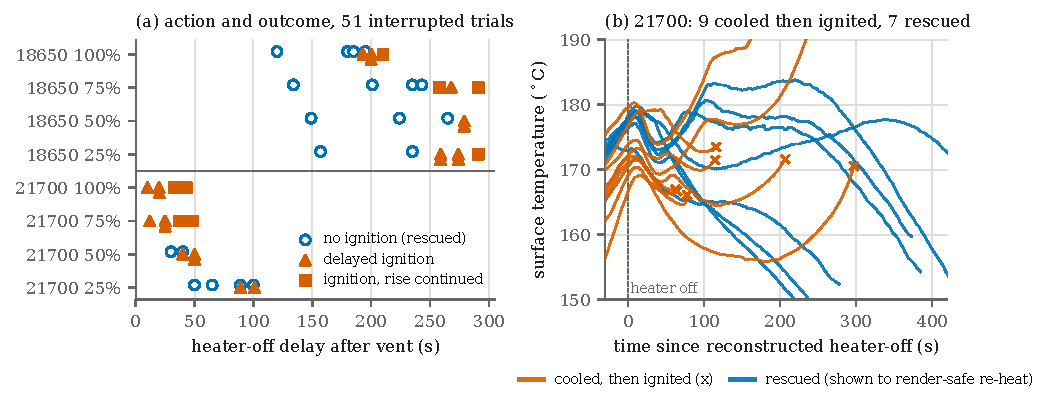
\includegraphics[width=\linewidth]{figures/fig_nist.pdf}
  \caption{NIST heat-interruption data \citep{nist2025heatdata,tam2026intervention}. (a) Heater-off delay after vent
  and the recorded outcome for every interrupted trial, by format and SOC. Two 21700 conditions contain no rescue at
  any tested delay. (b) The nine 21700 trials that cooled by at least 2\degC\ after heater-off and then ignited (x
  marks ignition), against the seven rescued 21700 trials, shown up to their render-safe re-heat. Surface temperature
  after heater-off does not order the risk. Heater-off is reconstructed with a 10~s thermocouple lag. Generated by
  \cmd{paper/make\_figures.py}.}
  \label{fig:nist}
\end{figure}

\subsection{Visual evidence for labels and timing}
Outcomes exist only as table cell colours in the paper (blue: no ignition; black: delayed ignition; red: ignition with
continued rise). We extracted them from the PDF's vector drawing layer, and independently had Muse Spark read rendered
images of Tables A1 and A2 (two calls). It returned 79 rows: the 77 experiments plus the two phantom rows. Its
outcome colours matched the vector extraction for 77 of 77 experiments, its delays for 51 of 51, and its SOC values for
77 of 77. Comparing the image reading, the vector extraction and the trace-derived outcome gave no three-way
disagreement on the 50 interrupted trials with traces. Exp~61 is labelled red but its trace cools by 6.8\degC\ before
igniting 78~s after heater-off; it behaves as a delayed ignition, which does not change the binary label.

Two of the paper's four supplementary videos show interrupted trials (S3: Exp~33; S4: Exp~81). They are edited
montages with speed-changed segments and burned-in captions. Muse Spark read the caption, an LED test timer and the
data-acquisition clock on 85 and 86 sampled frames, which places every frame on the acquisition clock; the speed
labels agreed with the clock to within 3.4\% and 3.8\% over 78 and 79 checks. Against that clock, the raw trace's
heater-off slope break lags the supply lamp going out by 6.96~s (S3) and 5.68~s (S4), and lags the start of the
edited ``Power Off'' segment by 9.89~s and 8.97~s. The thermocouple lag is therefore 6--10~s depending on the marker,
and heater-off is uncertain by about 3~s. The benchmark keeps the 10~s lag as a protocol parameter and adds a
sensitivity run at 7~s. SAM~3.1, prompted with a box over the jet, timed ignition onset in the videos; the trace's
ignition detector is later by $2.15 \pm 2.0$~s (S3) and $3.41 \pm 2.0$~s (S4), which corroborates it. SAM's onset was
one frame (0.03~s) after simple pixel counting in S3 and the same frame in S4: it added no precision for this task,
and we say so. The whole visual job cost \$0.70 on the Meta Model API. The model text and request hashes are kept; the
images are not redistributed.

\subsection{Task and actions}
At the reconstructed heater-off time of each interrupted trial with a trace, the agent receives the thermocouple trace
from power-on to heater-off, the cell's format, chemistry and capacity, the declared SOC, and the vent time, as an
external vent alarm would provide it. It outputs $P(\text{ignition})$ with an interval and one action:
\emph{stand down} (stopping the heat is enough), \emph{escalate} (suppress or evacuate), or \emph{observe}($W$) with
$W \in \{30, 60\}$~s, after which it sees $W$ more seconds of the recorded trace and must stand down or escalate.
Every action has an observed answer in the record, so the task is factual, not counterfactual. A stand-down on a trial
that ignited is an \emph{unsafe stand-down}; an escalation on a trial that was rescued is a \emph{missed rescue}. If a
trial ignites inside the watch window, an observe action on it counts as unsafe: the cell ignited while the agent
waited. Under the exploratory event reconstruction, 3 of the 31 ignited trials ignite within 30~s of heater-off and 12
within 60~s, so observation has a real price. Each policy reports the watch time it spent. Post-off features may come
only from the window the policy paid for.

The agent does not choose the heater-off time. Each trial records one stop time, chosen adaptively by the
experimenters, so an agent-chosen stop time could be scored only where it matches the recorded one, or under an
untestable assumption that stopping earlier never hurts the same cell. Even with that assumption, a held-out per-condition
lookup is identified on 8 of 51 trials; without it, 0--3 of 51 trials match any policy we tested.

\subsection{Sealed outcomes, committed before revealed}
At ingest the ledger records, for each trial, only a SHA-256 commitment, with a per-trial salt, over the outcome and
every field that scoring depends on: the ignition time, the flags (censored, inferred heater-off), the truncation
point and the source of each reconstructed event. An earlier seal covered the outcome alone, which left the ignition
time open to an undetected edit (Section~\ref{sec:system}). The plaintext lives in a sealed store the agent's tools
cannot read. A \emph{reveal} record (outcome
and salt) is written only after a decision for that trial is committed. The verifier gains two checks for campaigns
that contain these records: every scored decision's sequence number is lower than its trial's reveal, and every reveal
matches its seal. Tampering with an outcome or revealing before committing makes verification fail. Old record kinds
and their verification are unchanged.

\subsection{World models and decision policy}
The world model and the decision policy are separate. A world model returns $P(\text{ignition} \mid
\text{observations so far})$ with a bootstrap interval. The decision policy maps that probability, the action costs
and the remaining options to an action. Costs are fixed in the protocol: an unsafe stand-down costs 100, an ignition
while watching costs 100 whatever is decided afterwards, an unnecessary escalation (on a trial that was rescued) costs
10, watching costs 0.05 per second, and an abstention costs 10 as a deferred escalation. \emph{Escalating on a trial
that ignited costs 0.} That is an assumption, not an observation: the experiments recorded no suppression, so the
efficacy of escalation is unknown, and every cost in this paper carries it. Sensitivity runs set the unsafe and
watch-ignition cost to 50 and 200, keeping the others. The agent's policies use the cost-minimising rule, which
without observation escalates when $P(\text{ignition}) > 10/110 = 1/11$. The frozen baselines are scored as hard
classification rules, with a 0.5 cut on their probability; Section~\ref{sec:results} shows that this difference
matters.

World models come from declarative specifications: features, family, grouping, and an optional constraint such as
zero unsafe errors on the training folds. Features at decision time use only the trace up to heater-off and declared
metadata, drawn from a generic library (level, slopes and rises over several windows, curvature, time and rise since
vent, format, SOC, delay). The families are thresholds (pooled, per format, per condition), logistic regression, a
one-node lumped thermal model with Arrhenius self-heating, and a two-node core/surface model whose core temperature is
the hidden state. For the two-node model, kinetic priors come from the same condition's continuous-heating trials and
the state is fitted on the pre-off trace; it forecasts the outcome under each available action (stop now; observe $W$
then decide; and, for experiment design, a heater-off delay $d$ after vent). Every physics forecast is labelled
\texttt{simulated: true}, carries an interval, and is scored like any other world model. The gate refuses any claim
that cites a simulated outcome as evidence, any claim about an action that has no recorded outcome, and any claim on
fewer trials than the protocol minimum of 20.

\subsection{The agent loop and its hypotheses}
In an intervention campaign the planner (Muse Wonder) has tools to list trials without outcomes, get a trace up to
heater-off, compute features, propose a policy specification, evaluate it on revealed training data only, submit it
for held-out scoring, commit a decision, reveal, propose next experiments, and write a final answer. The pre-off data
are presented so that the planner can state competing mechanistic hypotheses, for example: the surface temperature
tracks the internal state; self-heating has passed a threshold that removing the heat cannot reverse; or the stored
energy (SOC) decides. Each hypothesis is recorded, and can name the policies that test it; in the final live run the planner named
them in the hypothesis text rather than linking them. The final answer is an operating
procedure (rule, the claim identifiers that support it, its limits) built only from supported claims. In the scripted
benchmark the benchmark code registers three hypotheses, each with an executable world model: \emph{surface} (surface
temperature tracks internal state; logistic regression on format and temperature at heater-off), \emph{self-heating}
(self-heating can continue after the heat stops; the two-node model), and \emph{SOC} (stored energy decides; logistic
regression on format, SOC and delay after vent). In its final live run the planner stated three of its own: surface temperature level and recent
slope reflect imposed heating that decays after the cut, so a high level alone may not mean self-sustaining ignition
(to be tested by threshold and thermal policies); internal self-heating persists after the cut and shows as positive
curvature and accelerating rise (two-node, curvature-logistic and observation policies); and SOC and the delay after
vent modulate the risk independently of the surface trajectory (SOC-aware logistic and table policies). It proposed
12 strategies to test them (Section~\ref{sec:live}). The same tools are exposed over MCP with write
access, under the same gate.

A Muse-only baseline gives the planner model the same pre-off summary with no tools and asks for the decision; it is
recorded and replayed like every other model call, and verification requires a provider receipt for each of its
decisions. The final Muse-only run recorded 64 model calls; replaying them without keys reproduces all 864 of its
ledger decisions.

\subsection{Screen funnel, gate claims and correction}
The agent may propose many candidate policies. Screening is cheap: cross-validation on the training folds of revealed
data. Only survivors are submitted for held-out scoring, and the protocol caps submissions at $K = 16$ before the
campaign starts. The unit counted against $K$ is an agent learning strategy; the frozen baselines are registered as
comparators and do not consume $K$. In the scripted benchmark the ledger records 3 strategies proposed, 1 screened out
(a constant-probability diagnostic) and 2 submitted (\texttt{agent\_threshold}, a search over single-feature
thresholds constrained to make no unsafe error on the training folds, and \texttt{agent\_logistic}, a search over
logistic models, including 30 and 60~s observation variants and one with the two-node physics forecast as a feature).
Inside those strategies, the inner cross-validation proposed 4{,}428 models and screened out 123. Nine baselines were
registered. Performance claims (``policy $P$ has $k$ unsafe stand-downs over $n$ held-out trials''; ``$P$ has lower
mean cost than $B$'') are a new gate claim kind recomputed only from committed decisions and revealed outcomes. A
comparison pairs two policies trial by trial and applies a two-sided sign-flip permutation test to the per-trial cost
differences (exact up to 20 nonzero differences, otherwise 100{,}000 seeded assignments with a plus-one correction),
Holm-corrected \citep{holm1979} over a family of submitted agent strategies times registered baselines, counted from
the ledger: $2 \times 9 = 18$. A baseline that has not been run (Muse-only, so far) enters the family with $p = 1$. An
exact McNemar test on unsafe stand-downs \citep{mcnemar1947} is reported as a descriptive secondary result.

In the prequential split the world model and the decision policy are each updated only after a reveal, and only if
the update passes a compatibility check recorded in the ledger: it adds no unsafe error on revealed trials and worsens
neither the five-bin expected calibration error nor the Brier score by more than 0.01. A rejected update is recorded
with its reason and not applied.

\subsection{Splits and the decision rule, fixed in advance}
The primary split is leave-one-condition-out (LOCO): eight folds, each holding out one format-and-SOC condition. The
secondary split is leave-one-format-out (LOFO), reported as a known transfer failure. A prequential split commits,
reveals and updates in experiment-number order \citep{dawid1984}. There is never a random trial split, because
replicates in a condition leak its boundary. Every analysis is run with and without the five inferred heater-off
trials, and with the thermocouple lag at 10~s and at 7~s; the cost-ratio sensitivities are run at 10~s with the
inferred trials. The registered primary analysis is LOCO, 10~s lag, inferred trials included, unsafe cost 100. All
other splits and variants are descriptive, even where the benchmark report computes a verdict for them.

The primary metric is the mean decision cost per trial, always shown with $n$, with a condition-block bootstrap 95\%
interval. Secondary metrics are unsafe stand-downs, missed rescues, Brier score \citep{brier1950}, log-loss, accuracy
with Wilson 95\% intervals \citep{wilson1927}, abstentions and their cost, and watch time spent.

\paragraph{Decision rule.} For each baseline $B$, we state that the agent's strategy $A$ beats $B$ only if $A$ has a
lower mean cost than $B$ under the primary analysis and the paired sign-flip test gives $p < 0.05$ after Holm
correction over the family of 18. A secondary two-part result requires an observed unsafe count no larger than $B$'s
and significantly fewer missed rescues by exact McNemar, in the same family; an observed non-increase in unsafe
stand-downs is not a test of non-inferiority. We report every pairwise result. Always-escalate makes no unsafe
stand-down by construction, so against it a strategy can win only by recovering rescues without adding unsafe
stand-downs. For any baseline that $A$ does not beat under this rule we say so; if it beats only weak ones, the
contribution of this section is the harness and the negative result.

\paragraph{Registration and its amendments.} The first registered endpoint was the count of unsafe stand-downs with an
exact McNemar test, Holm-corrected over submitted policies. Two amendments, recorded in the protocol record with their
reasons, changed it before the scoring runs reported here. Amendment~2 made the mean decision cost primary, with the
costs above, because under the first costs observation could never pay for itself and because McNemar on unsafe
counts cannot separate zero from three unsafe errors at 5\%. Amendment~3 counts only screened agent strategies
against $K$ and in the correction family, because frozen baselines are comparators, not strategies. Both were
committed on 29 October 2026 (UTC; 30 October in local time), amendment~2 about half an hour and amendment~3 31~s before the first scoring run under
them started. Earlier code could already score held-out decisions under the first endpoint, and the repository
history cannot show whether any held-out result was looked at before the amendments. The data are public, and the same
trials were analysed before the benchmark was fixed (Section~\ref{sec:exploratory}). We therefore do not describe the
analysis as pre-registered without these qualifications. We have not changed the split, the metric or the rule after
the scoring runs.

\paragraph{Power.} The rule is strict for 50 trials. With $d$ nonzero paired differences all favouring $A$, the best
exact two-sided $p$ is $2^{1-d}$, so $A$ needs at least 6 such trials for an unadjusted $p<0.05$ and at least 10 at
the first Holm step with 18 comparisons; mixed signs or unequal cost magnitudes need more. The descriptive McNemar test
on unsafe stand-downs cannot reach $p<0.05$ for zero against three unsafe errors: its best two-sided $p$ is 0.25. A
failure to beat a baseline is therefore weak evidence that the policies are equal.

\subsection{Exploratory analysis on the same trials (disclosed)}\label{sec:exploratory}
Before the benchmark was fixed, a data-validation analysis looked at the same 50 interrupted trials. It compared about
16 models under leave-one-trial-out (LOO), LOCO and LOFO; Table~\ref{tab:exploratory} shows a selection. Its findings
shaped the design: sensor features transferred across SOC within a format better than the per-condition delay lookup,
and nothing transferred across format. The choice of LOCO as the primary split was made knowing this. There is
therefore no untouched held-out set in this study. The benchmark's feature library is generic and does not contain the
exploratory best feature as a named input, but the authors' knowledge of it cannot be removed, and we report the
exploratory numbers as exploratory only.

\begin{table}[t]
\centering\small
\caption{Exploratory analysis on the 50 interrupted trials with traces (31 ignited, 19 rescued), before the benchmark
was fixed. Accuracy / unsafe stand-downs / missed rescues; Brier in the LOCO column. Thresholds were refit inside each
fold. Under LOCO the per-condition lookup falls back to a per-format threshold. Not a benchmark result.}
\label{tab:exploratory}
\setlength{\tabcolsep}{3pt}
\begin{tabular}{@{}lccc@{}}
\toprule
Model & LOO & LOCO (Brier) & LOFO \\
\midrule
Always predict ignition (= always escalate) & 0.62 / 0 / 19 & 0.62 / 0 / 19 (0.380) & 0.62 / 0 / 19 \\
Condition lookup (majority per format and SOC) & 0.48 / 11 / 15 & 0.44 / 11 / 17 (0.312) & 0.44 / 11 / 17 \\
Paper's Table-3 delay lookup & 0.76 / 4 / 8 & 0.66 / 6 / 11 (0.277) & 0.38 / 31 / 0 \\
Pooled temperature threshold, refit & 0.70 / 3 / 12 & 0.70 / 3 / 12 (0.229) & 0.48 / 7 / 19 \\
Logistic: format, SOC, delay & 0.66 / 2 / 15 & 0.58 / 6 / 15 (0.279) & 0.46 / 15 / 12 \\
Logistic: format, $T_\text{off}$, 30~s slope, 60~s rise & 0.82 / 4 / 5 & 0.86 / 2 / 5 (0.138) & 0.60 / 5 / 15 \\
30~s pre-off slope threshold (per condition or format) & 0.66 / 8 / 9 & 0.84 / 0 / 8 (0.145) & 0.62 / 7 / 12 \\
\bottomrule
\end{tabular}
\end{table}

Under LOCO, the sensor-and-format logistic model beat the delay lookup on paired trials, 14 against 4 discordant
($p = 0.031$), and the per-format slope threshold 11 against 2 ($p = 0.022$). Under LOO the difference was 7 against 4
($p = 0.55$): with replicates of the same condition in training, delay is as good as the sensor. Shuffling the sensor
features within condition and 20~s delay bin left a log-loss gain for the 30~s slope ($p = 0.02$, 200 permutations).
With about 16 models compared, none of these $p$-values survives correction. At $n = 50$, an accuracy of 0.86 has a
Wilson interval of about 0.74--0.93 and 0.66 of about 0.52--0.78, so unpaired differences below about 15 points are
noise. Within a condition, the recorded delay alone separates outcomes with 3 in-sample errors out of 50, and at the
boundary pairs (for example Exp~76 against Exp~77, both 21700 at 25\% with an 89~s delay) the temperature at heater-off
and the 30~s slope differ by less than 3.5\degC\ and 0.03\degC/s. A lumped one-node Arrhenius model fitted to each
trial's own pre-off trace fitted it to 0.4--2.0~K but forecast ``cools, no ignition'' for all 50 trials (31 unsafe);
with kinetics taken from the continuous trials the result was the same. Nine 21700 trials cooled by 2.8--14.6\degC\
after heater-off and then ignited 63--346~s later, while rescued 21700 cells re-rose to about 180\degC\ and held
(Figure~\ref{fig:nist}b): the surface temperature after interruption is not monotone in risk, and the hidden state is
internal.

\subsection{Results}\label{sec:results}
The scripted benchmark (\cmd{translucent bench nist}; report \cmd{evals/INTERVENE.md}, results
\cmd{evals/results/intervene-20261030T032322979014Z*.json}) ran all six registered variants under all three splits,
offline and with no provider call: 1{,}500 committed decisions per variant with the inferred trials, 1{,}350 without.
Every number below is recomputed by the gate from committed decisions and revealed outcomes. Every cost assumes that
escalating on a trial that ignited costs 0, because the efficacy of escalation was not observed. No policy abstained
in any variant. Muse-only was not run in the scripted benchmark, where it enters the correction family with
$p = 1$; its row comes from its final live run (Section~\ref{sec:live}), a separate ledger holding the same 50 trials
and the same frozen baselines, whose scores there equal those here exactly.

\begin{table}[t]
\centering\scriptsize
\caption{Registered primary analysis: LOCO, 10~s lag, inferred trials included, unsafe:escalation cost 10:1 (unsafe
stand-down or ignition while watching 100, unnecessary escalation 10, watching 0.05 per second; escalating on an
ignited trial costs 0, an unobserved assumption). Mean cost with condition-block bootstrap 95\% interval; accuracy
with Wilson 95\% interval. No policy abstained. Always-escalate's Brier score is that of a constant forecast of 1. $^\dagger$Final live
Muse-only run, in its own ledger with the same trials and frozen baselines.}
\label{tab:loco}
\setlength{\tabcolsep}{3pt}
\begin{tabular}{@{}lrlrrrrrl@{}}
\toprule
Policy & $n$ & Mean cost [95\%] & Unsafe & Missed & Watch s & Brier & Log-loss & Accuracy [95\%] \\
\midrule
\texttt{always\_escalate} & 50 & 3.80 [2.19, 5.10] & 0 & 19 & 0 & 0.380 & 2.63 & 0.62 [0.48, 0.74] \\
\texttt{paper\_table3} & 50 & 10.40 [3.98, 17.84] & 5 & 2 & 0 & 0.140 & 0.97 & 0.86 [0.74, 0.93] \\
\texttt{delay\_lookup\_refit} & 50 & 14.20 [1.50, 29.80] & 6 & 11 & 0 & 0.277 & 0.82 & 0.66 [0.52, 0.78] \\
\texttt{fixed\_temperature} & 50 & 27.60 [14.14, 43.88] & 13 & 8 & 0 & 0.257 & 0.71 & 0.58 [0.44, 0.71] \\
\texttt{temperature\_refit} & 50 & 8.40 [2.28, 15.69] & 3 & 12 & 0 & 0.229 & 0.67 & 0.70 [0.56, 0.81] \\
\texttt{physics\_only} & 50 & 62.00 [48.99, 78.08] & 31 & 0 & 0 & 0.620 & 4.28 & 0.38 [0.26, 0.52] \\
\texttt{two\_node\_physics} & 50 & 62.00 [48.99, 78.08] & 31 & 0 & 0 & 0.480 & 1.73 & 0.38 [0.26, 0.52] \\
\texttt{always\_observe\_30} & 50 & 14.26 [6.42, 22.16] & 6 & 4 & 1461 & 0.133 & 0.44 & 0.80 [0.67, 0.89] \\
\texttt{muse\_only}$^\dagger$ & 50 & 13.82 [3.03, 27.34] & 6 & 7 & 420 & 0.195 & 0.66 & 0.74 [0.60, 0.84] \\
\midrule
\texttt{agent\_threshold} & 50 & 3.80 [2.19, 5.10] & 0 & 19 & 0 & 0.203 & 0.61 & 0.62 [0.48, 0.74] \\
\texttt{agent\_logistic} & 50 & 3.72 [2.07, 5.12] & 0 & 18 & 120 & 0.152 & 0.47 & 0.64 [0.50, 0.76] \\
\bottomrule
\end{tabular}
\end{table}

\begin{table}[t]
\centering\scriptsize
\caption{Paired comparisons in the registered primary analysis (Table~\ref{tab:loco}). Nonzero: trials whose costs
differ. $p$: two-sided sign-flip test on per-trial cost differences ($10^{-5}$ is the Monte Carlo floor of 100{,}000
assignments). Holm over the family of 18 (2 submitted strategies $\times$ 9 registered baselines; the not-run
Muse-only comparator enters with $p=1$). McNemar on unsafe stand-downs is descriptive. ``Rule'': the registered
decision rule is met. Costs assume escalation on an ignited trial costs 0, an unobserved assumption.}
\label{tab:pairs}
\setlength{\tabcolsep}{4pt}
\begin{tabular}{@{}llrrrrrc@{}}
\toprule
Strategy & Baseline & Mean cost & Nonzero & $p$ & Holm $p$ & Unsafe McNemar $p$ & Rule \\
\midrule
\texttt{agent\_threshold} & \texttt{always\_escalate} & 3.80 / 3.80 & 0 & 1 & 1 & 1 & no \\
 & \texttt{paper\_table3} & 3.80 / 10.40 & 22 & 0.16 & 1 & 0.062 & no \\
 & \texttt{delay\_lookup\_refit} & 3.80 / 14.20 & 14 & 0.031 & 0.38 & 0.031 & no \\
 & \texttt{fixed\_temperature} & 3.80 / 27.60 & 24 & 0.00027 & 0.0035 & 0.00024 & yes \\
 & \texttt{temperature\_refit} & 3.80 / 8.40 & 10 & 0.25 & 1 & 0.25 & no \\
 & \texttt{physics\_only} & 3.80 / 62.00 & 50 & $10^{-5}$ & 0.00018 & $9.3\times10^{-10}$ & yes \\
 & \texttt{two\_node\_physics} & 3.80 / 62.00 & 50 & $10^{-5}$ & 0.00018 & $9.3\times10^{-10}$ & yes \\
 & \texttt{always\_observe\_30} & 3.80 / 14.26 & 50 & 0.032 & 0.38 & 0.031 & no \\
\midrule
\texttt{agent\_logistic} & \texttt{always\_escalate} & 3.72 / 3.80 & 5 & 1 & 1 & 1 & no \\
 & \texttt{paper\_table3} & 3.72 / 10.40 & 23 & 0.13 & 1 & 0.062 & no \\
 & \texttt{delay\_lookup\_refit} & 3.72 / 14.20 & 17 & 0.031 & 0.38 & 0.031 & no \\
 & \texttt{fixed\_temperature} & 3.72 / 27.60 & 27 & 0.00021 & 0.0029 & 0.00024 & yes \\
 & \texttt{temperature\_refit} & 3.72 / 8.40 & 13 & 0.25 & 1 & 0.25 & no \\
 & \texttt{physics\_only} & 3.72 / 62.00 & 49 & $10^{-5}$ & 0.00018 & $9.3\times10^{-10}$ & yes \\
 & \texttt{two\_node\_physics} & 3.72 / 62.00 & 49 & $10^{-5}$ & 0.00018 & $9.3\times10^{-10}$ & yes \\
 & \texttt{always\_observe\_30} & 3.72 / 14.26 & 50 & 0.032 & 0.38 & 0.031 & no \\
\bottomrule
\end{tabular}
\end{table}

\paragraph{The primary result is negative.} Neither strategy beats always escalating (Table~\ref{tab:pairs}).
\texttt{agent\_threshold} takes the same action as always-escalate on all 50 trials: in every fold the search chose a
threshold constrained to make no unsafe error in training, and the probability on its stand-down side never fell
below the 1/11 escalation threshold. \texttt{agent\_logistic} differs from always-escalate on 5 trials: one correct
stand-down (Exp~22, $-10$) and four 30~s watches that ended in escalation (Exp~74, 75, 77 and 78, $+1.5$ each), for
3.72 against 3.80 per trial, $p = 1$. Its forecasts are informative: its Brier score (0.152) is lower than every
baseline's except the in-sample Table-3 lookup (0.140) and the always-observe policy, which sees 30~s more of every
trace (0.133). But under a 10:1 cost ratio almost no held-out probability falls low enough to stand down, so the
forecasts barely change the actions.

\paragraph{Outcome of the decision rule, per baseline.} Against always-escalate, the paper's Table-3 lookup, the
refitted delay lookup, the refitted temperature threshold and always-observe-30, neither strategy meets the rule; the
smallest Holm-corrected $p$ is 0.38. Against the fixed 170\degC\ threshold, the one-node model and the two-node
model, both strategies meet it (Holm $p \le 0.0035$). The secondary two-part result (no more unsafe stand-downs and
significantly fewer missed rescues) is met against no baseline. Muse-only entered this family with $p = 1$ because it was not run here; its live run
is in another ledger, so we make no paired claim against it from the scripted strategies.

\paragraph{What the three registered wins mean.} They are the registered computation, and an independent audit
recomputed every cost, test and correction exactly. They do not show that the agent learned anything, for four
reasons, all found after scoring. We made each one formal as a post-hoc sensitivity analysis, recorded in the same
ledger, re-checked by the verifier and kept outside the registered family (Table~\ref{tab:posthoc}). None of them
can support a new gate claim or replace the registered result.
\begin{enumerate}
  \item \emph{Decision-rule asymmetry.} The strategies use the cost rule; the baselines use a 0.5 cut. Rescoring each
  probabilistic baseline's originally committed probabilities under the cost rule, with no refit and no watching,
  brings the fixed-threshold, refitted-threshold and delay-lookup baselines to 3.80, the cost of always escalating,
  and the agents' advantage over them to $p = 1$. The two-node model falls from 62.0 to 12.4, and the agents' margin
  over it is short of significance even before correction ($p = 0.062$). Only the one-node model, which forecasts zero
  for every trial, stays at 62.0. The Table-3 lookup is a hard 0/1 rule and is unchanged.
  \item \emph{An illustrative threshold on a cliff.} The fixed baseline's 170\degC\ has no documented source; we treat
  it as illustrative. A sweep from 140 to 200\degC\ in 5\degC\ steps (Table~\ref{tab:sweep}) shows how sharply its
  errors change with the cut: 3 unsafe stand-downs at 160\degC, 13 at 170\degC.
  \item \emph{Physics baselines that do not discriminate.} The one-node model forecasts $P(\text{ignition}) = 0$ on
  every trial; the two-node model forecasts at most 0.25. Under the 0.5 cut both stand down on all 50 trials and make
  31 unsafe stand-downs, so any policy that escalates beats them.
  \item \emph{Dependence within conditions.} Under LOCO the decisions in a held-out condition share one fitted model,
  and outcomes cluster by condition. The registered test flips signs per trial. A test that flips signs per
  condition has 8 blocks, so its smallest two-sided $p$ is $2/2^8 = 0.0078$, or 0.14 at the first Holm step of 18.
  That is exactly what both agents reach against the physics baselines; against the fixed threshold they reach
  $p = 0.031$, Holm 0.44. No clustered comparison survives correction.
\end{enumerate}
The reading the evidence supports is narrower than the registered verdicts: a cost-aware rule beats 0.5-cut rules
under a 10:1 cost asymmetry, and the learned world models add nothing measurable over always escalating.

\begin{table}[t]
\centering\small
\caption{Post-hoc sensitivities for the registered primary analysis, outside the registered family. Registered:
per-trial sign-flip $p$ and Holm (as in Table~\ref{tab:pairs}). Clustered: sign flips over the 8 condition blocks,
with Holm over the same family of 18. Cost rule: the baseline's committed probabilities rescored under the agents'
cost rule, and the agent's unadjusted $p$ against that version. ``n/a'': the baseline has no probability to rescore
(always-escalate is already constant; always-observe has its own continuation rule). Costs assume escalation on an
ignited trial costs 0.}
\label{tab:posthoc}
\setlength{\tabcolsep}{4pt}
\begin{tabular}{@{}llrrrrrr@{}}
\toprule
& & \multicolumn{2}{c}{Registered} & \multicolumn{2}{c}{Clustered} & \multicolumn{2}{c}{Cost rule} \\
\cmidrule(lr){3-4}\cmidrule(lr){5-6}\cmidrule(l){7-8}
Strategy & Baseline & $p$ & Holm & $p$ & Holm & Baseline cost & $p$ \\
\midrule
\texttt{agent\_threshold} & \texttt{always\_escalate} & 1 & 1 & 1 & 1 & n/a & n/a \\
 & \texttt{paper\_table3} & 0.16 & 1 & 0.125 & 1 & 10.40 & 0.16 \\
 & \texttt{delay\_lookup\_refit} & 0.031 & 0.38 & 0.50 & 1 & 3.80 & 1 \\
 & \texttt{fixed\_temperature} & 0.00027 & 0.0035 & 0.031 & 0.44 & 3.80 & 1 \\
 & \texttt{temperature\_refit} & 0.25 & 1 & 0.50 & 1 & 3.80 & 1 \\
 & \texttt{physics\_only} & $10^{-5}$ & 0.00018 & 0.0078 & 0.14 & 62.00 & $10^{-5}$ \\
 & \texttt{two\_node\_physics} & $10^{-5}$ & 0.00018 & 0.0078 & 0.14 & 12.40 & 0.062 \\
 & \texttt{always\_observe\_30} & 0.032 & 0.38 & 0.078 & 0.86 & n/a & n/a \\
\midrule
\texttt{agent\_logistic} & \texttt{always\_escalate} & 1 & 1 & 1 & 1 & n/a & n/a \\
 & \texttt{paper\_table3} & 0.13 & 1 & 0.125 & 1 & 10.40 & 0.13 \\
 & \texttt{delay\_lookup\_refit} & 0.031 & 0.38 & 0.50 & 1 & 3.80 & 1 \\
 & \texttt{fixed\_temperature} & 0.00021 & 0.0029 & 0.031 & 0.44 & 3.80 & 1 \\
 & \texttt{temperature\_refit} & 0.25 & 1 & 0.50 & 1 & 3.80 & 1 \\
 & \texttt{physics\_only} & $10^{-5}$ & 0.00018 & 0.0078 & 0.14 & 62.00 & $10^{-5}$ \\
 & \texttt{two\_node\_physics} & $10^{-5}$ & 0.00018 & 0.0078 & 0.14 & 12.40 & 0.062 \\
 & \texttt{always\_observe\_30} & 0.032 & 0.38 & 0.063 & 0.75 & n/a & n/a \\
\bottomrule
\end{tabular}
\end{table}

\begin{table}[t]
\centering\small
\caption{Post-hoc sweep of the fixed temperature threshold, registered primary analysis (50 trials): stand down if
the temperature at heater-off is at or below the threshold. Descriptive; no threshold is selected from it, and the
registered baseline stays at 170\degC. Costs assume escalation on an ignited trial costs 0.}
\label{tab:sweep}
\setlength{\tabcolsep}{5pt}
\begin{tabular}{@{}lrrrrrrrrrrrrr@{}}
\toprule
Threshold (\degC) & 140 & 145 & 150 & 155 & 160 & 165 & 170 & 175 & 180 & 185 & 190 & 195 & 200 \\
\midrule
Unsafe & 0 & 0 & 0 & 0 & 3 & 9 & 13 & 22 & 27 & 31 & 31 & 31 & 31 \\
Missed & 18 & 17 & 14 & 12 & 10 & 8 & 8 & 6 & 0 & 0 & 0 & 0 & 0 \\
Mean cost & 3.6 & 3.4 & 2.8 & 2.4 & 8.0 & 19.6 & 27.6 & 45.2 & 54 & 62 & 62 & 62 & 62 \\
\bottomrule
\end{tabular}
\end{table}

\paragraph{A threshold chosen after the fact beats every agent.} At 155\degC\ the sweep reaches a mean cost of 2.4
with no unsafe stand-down, lower than every agent strategy, scripted (3.72, 3.80) or live (best 3.00 and 3.40). That number is
in sample: the threshold was picked by looking at the held-out outcomes it is scored on, and 5\degC\ higher it makes
3 unsafe stand-downs. It does not show that 155\degC\ is a safe operating point. It shows how little separation the
data allow: a single cut on the surface temperature, tuned with hindsight, beats every learned policy, and the
margin between it and a cut that stands down on a cell that then ignites is one sweep step. Any policy reported on
these 50 trials, ours included, has to be read against that.

\begin{table}[t]
\centering\small
\caption{The same policies under LOFO and the prequential split (10~s lag, inferred trials included, 50 trials):
mean cost / unsafe stand-downs / missed rescues. Descriptive. Costs assume escalation on an ignited trial costs 0.}
\label{tab:lofo}
\setlength{\tabcolsep}{4pt}
\begin{tabular}{@{}lrrrrrr@{}}
\toprule
& \multicolumn{3}{c}{LOFO} & \multicolumn{3}{c}{Prequential} \\
\cmidrule(lr){2-4}\cmidrule(l){5-7}
Policy & Cost & Unsafe & Missed & Cost & Unsafe & Missed \\
\midrule
\texttt{always\_escalate} & 3.80 & 0 & 19 & 3.80 & 0 & 19 \\
\texttt{paper\_table3} & 10.40 & 5 & 2 & 10.40 & 5 & 2 \\
\texttt{delay\_lookup\_refit} & 62.00 & 31 & 0 & 42.80 & 21 & 4 \\
\texttt{fixed\_temperature} & 27.60 & 13 & 8 & 27.80 & 13 & 9 \\
\texttt{temperature\_refit} & 17.80 & 7 & 19 & 15.60 & 7 & 8 \\
\texttt{physics\_only} & 62.00 & 31 & 0 & 62.00 & 31 & 0 \\
\texttt{two\_node\_physics} & 62.00 & 31 & 0 & 62.00 & 31 & 0 \\
\texttt{always\_observe\_30} & 25.66 & 11 & 11 & 19.06 & 8 & 8 \\
\texttt{muse\_only} & \multicolumn{6}{l}{not run (live runs used LOCO only)} \\
\midrule
\texttt{agent\_threshold} & 16.40 & 7 & 12 & 6.20 & 2 & 11 \\
\texttt{agent\_logistic} & 3.83 & 0 & 19 & 4.49 & 1 & 12 \\
\bottomrule
\end{tabular}
\end{table}

\paragraph{LOFO and prequential.} Across format nothing transfers (Table~\ref{tab:lofo}). \texttt{agent\_threshold}
makes 7 unsafe stand-downs; \texttt{agent\_logistic} avoids them only by escalating on every trial (one 30~s watch);
the refitted delay lookup stands down on every trial. In the prequential split both strategies make unsafe stand-downs
(2 and 1) and neither is cheaper than always escalating. The compatibility check accepted 343 and rejected 147
proposed updates across all policies; for the strategies it accepted 22 and rejected 27 (\texttt{agent\_threshold})
and accepted 20 and rejected 29 (\texttt{agent\_logistic}), every rejection by the calibration guard. The 16 rejections for adding an unsafe error on revealed trials were all
for the refitted delay lookup (9) and always-observe-30 (7). Rejected updates are recorded and were not applied.

\begin{table}[t]
\centering\small
\caption{Registered sensitivities, LOCO: mean cost (unsafe / missed), and each strategy's $p$ / Holm $p$ against
always-escalate. Lag and inclusion variants use unsafe cost 100; cost ratios use 10~s and the inferred trials.
Descriptive; the first row is the primary analysis. Costs assume escalation on an ignited trial costs 0, an
unobserved assumption.}
\label{tab:sens}
\setlength{\tabcolsep}{2.5pt}
\begin{tabular}{@{}lrlllll@{}}
\toprule
Variant & $n$ & Always escalate & \texttt{agent\_threshold} & \texttt{agent\_logistic} & thr.\ vs esc. & log.\ vs esc. \\
\midrule
10~s, with inferred, 10:1 & 50 & 3.80 (0/19) & 3.80 (0/19) & 3.72 (0/18) & 1 / 1 & 1 / 1 \\
10~s, without inferred & 45 & 4.22 (0/19) & 4.22 (0/19) & 3.33 (0/15) & 1 / 1 & 0.125 / 1 \\
7~s, with inferred & 50 & 3.80 (0/19) & 3.80 (0/19) & 3.88 (0/17) & 1 / 1 & 0.78 / 1 \\
7~s, without inferred & 45 & 4.22 (0/19) & 4.22 (0/19) & 3.33 (0/15) & 1 / 1 & 0.125 / 1 \\
Unsafe cost 50 (5:1) & 50 & 3.80 (0/19) & 6.00 (4/10) & 2.80 (0/14) & 0.38 / 1 & 0.062 / 0.62 \\
Unsafe cost 200 (20:1) & 50 & 3.80 (0/19) & 3.80 (0/19) & 3.80 (0/19) & 1 / 1 & 1 / 1 \\
\bottomrule
\end{tabular}
\end{table}

\paragraph{Sensitivity.} No variant changes the conclusion (Table~\ref{tab:sens}). In no variant does either strategy
beat always escalating; the closest is \texttt{agent\_logistic} at an unsafe cost of 50, 2.80 against 3.80 with
unadjusted $p = 0.062$ and Holm $p = 0.62$, where \texttt{agent\_threshold} is worse than always escalating (4 unsafe
stand-downs). At an unsafe cost of 200 both strategies become always-escalate. The registered wins over the fixed
threshold and the two physics models recur in every variant, for the reasons above. The without-inferred variant is
not a neutral data-quality check. All five inferred trials ignited, and the flag is a function of early ignition: a
heater-off time is inferred when no clear slope break is found well before ignition, which happens when ignition
follows heater-off quickly. Excluding them drops 5 of 31 ignitions by an outcome-linked rule. Their decision points are
placed by a different procedure (the condition's mean vent time plus the delay), and all five ignite within 60~s of
it, three within 30~s, so they hand every watching policy a near-certain ignition while watching: three of
always-observe-30's six unsafe outcomes in the primary analysis. The scripted strategies never read the flag. It was visible to the planner, and in the
Muse-only prompt, in the first live runs; since then every quality flag is hidden from the planner's view of the
trials and from both Muse-only prompt stages, and remains only in the sealed evidence and the audit export.

\paragraph{Two-node physics.} Scored as a world model under LOCO, the two-node model has Brier 0.480 and log-loss 1.73,
against 0.620 and 4.28 for the one-node model; both are worse than a constant forecast of the base rate would be
(Brier $0.62 \times 0.38 = 0.236$, computed in sample). It does not discriminate ignition from rescue, and its
alternative-action forecasts are simulated and support no claim. As a feature inside training folds it does slightly
better. \texttt{agent\_logistic}'s search included a logistic model on format, temperature at heater-off and the
two-node forecast. In all 8 LOCO folds that model had a lower inner cross-validation Brier score than the same model
without the physics feature, and in 2 folds a lower inner cost. In every LOCO and LOFO fold, however, a sensor-feature model
without it had a lower or equal inner cost and was selected, so the physics feature contributed to no held-out
decision. Under LOCO its kinetic priors come from the held-out condition's continuous-heating trials: these are
separate trials, but the information is condition-specific.

\paragraph{Operating procedure.} The gate supported an operating procedure built on \texttt{agent\_threshold}, from
three supported performance claims (\texttt{int\_2676cb8a}, \texttt{int\_12956688}, \texttt{int\_2cc88d76}): 0 unsafe
stand-downs and 19 missed rescues over 50 held-out trials under LOCO (mean cost 3.8), 7 and 12 under LOFO (16.4), and
2 and 11 prequentially (6.2). Its rule: at recorded heater-off apply the declared world model and the registered cost
rule; if it selects observation, commit the 30 or 60~s watch, use only the paid samples, and commit stand-down or
escalation before the outcome is revealed. Its recorded limits are that only the recorded heater-off was observed and
neither suppression efficacy nor alternative stop times were; that it rests on 50 interrupted traces from one study
and is a case study, not a validated fire-safety procedure; that one surface thermocouple was used, internal state was
not measured and events were reconstructed with a 10~s lag; that rescues are censored and some heater-off times
inferred; that format transfer fails; and that a supported count of observed errors is not a guarantee of safe
stand-down. Under LOCO this procedure acts exactly as always escalating. The gate supports it as a description of
observed errors, which is all a supported claim here means.

\paragraph{Offline verification.} Run on the exported primary campaign, \cmd{translucent verify}
re-checks 126 of 126 findings, finds 247 of 247 files intact and
re-derives 1{,}500 decisions, with no problems
(fixture \cmd{web/public/fixtures/nist-bench.json}). It refits every model and re-screens every candidate on the way,
and also recomputes the 57 post-hoc score records and 90 post-hoc comparison records above, so they are as
tamper-evident as the registered ones. It took 67~s on one core of a Linux server and 2~min 47~s on a Windows laptop
under other load, with no provider keys. Every one of the six variants verifies (8{,}700 decision checks, 756
findings). The independent audit ran the full benchmark again and found no difference from the
committed results in any field across all six variants. In its leakage tests, for three held-out groups, it flipped every
held-out outcome and ignition time and added 40\degC\ to every post-heater-off sample of the held-out trials; no
held-out decision made before a paid watch changed. The audit used an earlier run of the benchmark, before the verifier fixes; every registered score of the run
reported here is identical to it in every variant, split and subset.

\subsection{Live campaigns with the Muse Wonder planner}\label{sec:live}
In the live campaigns Muse Wonder states the hypotheses, proposes and submits the strategies, and writes the claims,
through the same tools and gate; the Muse-only baseline runs in its own campaign. Both are LOCO on the same 50
trials. We ran each twice. The first runs used code from before the verifier fixes of Section~\ref{sec:system}; the
final runs used the final code. Between them four things changed: the nine frozen baselines are registered in the
live ledger, so the gate tests the planner's strategies against them directly (the first planner run could compare
its strategies only with its own constant-escalation policy, in a family of 10); the inferred heater-off flag, which
marks ignition in 5 of 5 trials, is hidden from the planner and from the Muse-only prompt; the outcome seal covers
every outcome-dependent field and verification refits every model; and the planner's step cap rose from 40 to 120,
with each fresh fold told that registration is frozen.

\begin{table}[t]
\centering\footnotesize
\caption{Live LOCO campaigns, 50 trials: unsafe stand-downs, missed rescues, mean cost, watch seconds, and the
paired sign-flip test against always-escalate (3.80; 0 unsafe, 19 missed). Final planner run: family of 90 (10
submitted strategies $\times$ 9 baselines). First planner run: only its best strategy was tested, against its own
constant escalation, in a family of 10. Muse-only runs are separate campaigns. Costs assume escalation on an ignited
trial costs 0. Recomputed from the committed decisions with the benchmark's scorer.}
\label{tab:live}
\setlength{\tabcolsep}{4pt}
\begin{tabular}{@{}lrrrrl@{}}
\toprule
Strategy & Unsafe & Missed & Mean cost & Watch s & $p$ (Holm) \\
\midrule
\multicolumn{6}{@{}l}{\emph{Final planner run (12 proposed, 2 screened out, 10 submitted)}} \\
\texttt{logistic\_curvature} (procedure) & 0 & 17 & 3.40 & 0 & 0.50 (1) \\
\texttt{logistic\_soc\_delay}, \texttt{logistic\_pooled\_all}, \texttt{search\_generic} & 0 & 17 & 3.40 & 0 & 0.50 (1) \\
\texttt{logistic\_observe60} & 0 & 15 & 3.54 & 540 & 0.40 (1) \\
\texttt{surface\_threshold\_level}, \texttt{constant\_escalate\_agent} & 0 & 19 & 3.80 & 0 & 1 (1) \\
\texttt{logistic\_observe30} & 1 & 15 & 5.51 & 510 & 0.78 (1) \\
\texttt{thermal\_observe30} & 4 & 6 & 9.71 & 510 & 0.13 (1) \\
\texttt{table3\_soc} & 5 & 2 & 10.40 & 0 & 0.16 (1) \\
\midrule
\multicolumn{6}{@{}l}{\emph{First planner run, pre-fix code (12 proposed, 2 screened out, 10 submitted)}} \\
\texttt{condition\_grouped\_logistic} (procedure) & 0 & 15 & 3.00 & 0 & 0.125 (1) \\
\texttt{full\_logistic} & 0 & 16 & 3.20 & 0 & --- \\
\texttt{surface}, \texttt{selfheat}, \texttt{format\_grouped} logistic & 0 & 17 & 3.40 & 0 & --- \\
\texttt{observe60\_logistic} & 0 & 15 & 3.54 & 540 & --- \\
\texttt{soc\_logistic} & 0 & 18 & 3.60 & 0 & --- \\
\texttt{constant\_high}, \texttt{surface\_threshold} & 0 & 19 & 3.80 & 0 & --- \\
\texttt{observe30\_logistic} & 1 & 16 & 5.71 & 510 & --- \\
\midrule
\texttt{muse\_only}, final run & 6 & 7 & 13.82 & 420 & --- \\
\texttt{muse\_only}, first run & 4 & 5 & 9.51 & 510 & --- \\
\bottomrule
\end{tabular}
\end{table}

\paragraph{The planner's result is the scripted result.} In the final run the planner's best strategies make no unsafe
stand-down and recover two rescues more than always escalating: 3.40 against 3.80, $p = 0.5$, Holm $p = 1$
(Table~\ref{tab:live}). In the first run the best was 3.00, $p = 0.125$, Holm $p = 1$, and that strategy was named in
the procedure after held-out scoring, which makes the point estimate optimistic. Neither run beats always escalating.
In both, the two physics-based strategies were screened out on the training folds (25 to 29 unsafe errors per fold;
27 in 43 training trials on the first), and in the final run the planner also submitted the paper's in-sample Table-3 lookup as one of its own
strategies; it made 5 unsafe stand-downs. Recomputed from the ledger, most of the planner's strategies, including its own
constant escalation, have Holm $p < 0.05$ against the fixed threshold and both physics baselines. The planner made no
such claim, and these comparisons mean as little as in the scripted benchmark: a policy that always escalates
``beats'' the fixed threshold (Holm $p = 0.018$).

\paragraph{The gate refused the planner's claim.} The final planner run proposed 18 claims. The gate supported 2: that
\texttt{logistic\_curvature} and \texttt{logistic\_pooled\_all} each made 0 unsafe stand-downs over 50 held-out trials.
It refused 15 because they were proposed before every held-out trial had been decided (for example ``7 of 50 registered
physical trials; 43 missing''). One was the planner's claim that \texttt{logistic\_curvature} beats always escalating;
the gate found it inconclusive: ``Mean decision cost 3.4 vs 3.8; paired sign-flip $p=0.5$, Holm $p=1$, family 90''.
The operating procedure the planner wrote, for \texttt{logistic\_curvature}, cites only the supported performance
claim. This is the gate doing what it is for: the model asserted a capability, and fixed code recomputed the claim
from committed decisions and declined it. In the first run, 8 of the planner's 12 claims were malformed and the gate
rejected them with bare missing-field errors, and a ninth was refused for incomplete held-out coverage; claim schemas
now name the missing fields.

\paragraph{Muse alone.} Asked for the decision with no tools, Muse Wonder made 4 unsafe stand-downs in the first run
(9.51 per trial) and 6 in the final run (13.82). The two runs used different prompts (the inferred flag was visible in
the first), so the difference is not run-to-run variance alone. In both campaigns the procedure policy the planner
wrote made none. Paired by trial across the two campaigns, a pairing chosen post hoc, after both runs, the final procedure
against Muse alone is 0 against 6
unsafe stand-downs, a mean difference of $-10.42$ per trial and an exact sign-flip $p = 0.031$; in the first
campaigns it is 0 against 4, $-6.51$ and $p = 0.125$. The pattern replicates, but it is post hoc and descriptive. The
comparison was not registered as a single test; in the registered family of 90 the Holm-corrected $p$ is 1; a handful of 100-cost
events dominates it at $n = 50$; and other planner-chosen strategies did make unsafe stand-downs (up to 5). We do not
claim that the harness makes the model's decisions safe. We report that the model on its own made unsafe stand-downs
in both runs and that the procedures built through the gate did not.

\paragraph{Verification, replay and spend.} \cmd{translucent verify} on the final planner ledger re-checks 18 of 18
findings, 247 files and 900 decisions (17~s); on the final Muse-only ledger, 76 files and 450 decisions. Replaying the
recorded model calls without provider keys reproduces all 1{,}343 planner-ledger decisions and all 864 Muse-only
decisions. Meta Model API spend, priced from each call's own tokens: planner \$3.96 (first run, 78 model calls and 276
tool calls) and \$3.74 (final run, 38 model calls); Muse-only \$2.98 in each run (64 model calls in the final run).
The whole project, both demonstrations included, has spent about \$32 of its \$145 hard cap; the scripted benchmark
made no provider call.

\paragraph{Process lessons.} Two failures are on record. A first planner attempt with a 40-step cap stopped inside
the first fold before any held-out decision, after \$0.27; its ledger is kept, and the cap is now 120. And when the
final planner and Muse-only campaigns ran in parallel, each charged the other's calls through the shared provider
balance, so the campaign records showed \$4.65 and \$8.54. The fix (commit \texttt{aac461e}) charges each call its own
tokens; the provider-side cap was never affected, and the figures above are token-priced.

\subsection{Next experiments by mechanism discrimination}
The agent proposes next experiments as a condition plus a heater-off delay after vent. They are ranked by how
strongly the recorded hypotheses' world models disagree about the outcome (the expected reduction in posterior
uncertainty over which hypothesis holds), not by outcome uncertainty alone. Each proposal records every hypothesis's
predicted $P(\text{ignition})$, is labelled simulated and proposed, and comes with a schedule a person can review:
heater on at 41~W; detect vent; heater off at vent $+\,d$; watch for at least 400~s; re-heat to render safe only after
that. No proposal is run or presented as observed.

In the scripted benchmark the three top-ranked proposals, scored by the Jensen--Shannon divergence between the three
equally weighted hypotheses' Bernoulli forecasts, are all 21700 cells: at 50\% SOC with heater-off 120~s after vent
(0.51~bits; surface 0.81, self-heating 0.00, SOC 0.79), at 100\% SOC and 120~s (0.48~bits; 0.93, 0.13, 0.91), and at
50\% SOC and 80~s (0.44~bits; 0.76, 0.00, 0.70). Every forecast is simulated; these are proposals, not observations. The ranking is weak evidence: nearly all the disagreement comes from the
self-heating hypothesis, whose two-node world model forecasts near-zero ignition everywhere and was shown above not to
discriminate, while the two statistical hypotheses agree with each other. A proposal ranked this way tests the
physics model more than it separates mechanisms.

% ======================================================================================================== 6
\section{Limitations}\label{sec:limits}

\paragraph{No untouched held-out set.} The exploratory analysis of Section~\ref{sec:exploratory} used the same 50
trials and informed the choice of the primary split. Every Demonstration~2 result is conditional on that.

\paragraph{Amended registration.} The primary endpoint and correction family were amended twice on the day of
scoring, the last time 31~s before the first scoring run under it, and earlier code could already score held-out
decisions (Section~\ref{sec:demo2}). The amendments did not change the conclusion: no strategy beats always
escalating under either endpoint.

\paragraph{An unequal comparison.} The agent's strategies use the cost rule and the baselines a 0.5 cut, the fixed
temperature threshold has no documented source, and both physics baselines stand down on every trial. The three
registered wins rest on these choices, not on what the agent learned (Section~\ref{sec:results}). The registered test
also treats trials as independent although they cluster by condition; with eight conditions, no comparison could
survive a clustered test.

\paragraph{Escalation is assumed to work.} Every cost assumes that escalating on a trial that ignited costs nothing.
The experiments recorded no suppression, so a missed rescue is the only price of escalating that the data can show.

\paragraph{Small, unextendable data.} The intervention benchmark has 50 scored trials in eight conditions of 5--8
trials each; one trial moves accuracy by 2 points. The decision rule is underpowered (Section~\ref{sec:demo2}). The
inferred heater-off flag marks five trials that all ignited, so the without-inferred sensitivity selects on the
outcome.
Nothing transfers across cell format in the exploratory analysis (LOFO accuracy at or below 0.62 at the estimated
heater-off, against 0.62 for always escalating).

\paragraph{Reconstructed events.} Vent, heater-off and ignition times are reconstructed from one surface thermocouple
at 1~Hz, calibrated on two edited videos. Heater-off is uncertain by about 3~s; five heater-off times are inferred.
The outcome labels come from table colours, read three ways with no disagreement, but the paper is internally
inconsistent in one place (Exp~44's colour against its Table~3 safe time), and we used the colour.

\paragraph{What cannot be claimed.} The data cannot show the outcome for the same cell under a different stop time; an
optimal or latest safe stop time per cell; any probability finer than about $\pm$15 points per condition; anything
about stopping before vent, 21700 rescue at 75--100\% SOC, other heater powers, other abuse modes, packs or modules,
forced convection, or other cell makes; internal state, which no sensor recorded; vent timing from the videos; or that
rescued cells stayed stable beyond their watch windows of 224--1000~s. Our claims stay within NIST's cells, heater
power and sensor.

\paragraph{Demonstration 1.} The planted mistakes are ours, so 24 of 24 measures coverage of the faults we thought of,
not of all faults. The clean growth-speed case uses a scripted filament on a real clock and scale, because only junk
point-prompt masks are recorded for Movie~4. Merged outlines have no cheap general rule yet. The second opinion and
the memory mechanism both have measured weaknesses (Section~\ref{sec:demo1}). The model-reviewer comparison used one
open model at one reasoning setting.

\paragraph{Scope of the guarantee.} The gate decides whether recorded evidence supports a finding; it does not
establish that a battery is safe. Verification proves the record is internally consistent and that decisions preceded
reveals; it cannot prove that the recordings themselves are faithful to the experiment. Its strength is limited by
the checks it runs: an earlier version accepted four kinds of forged intervention record, and we know of those only
because a review built them. The reconstructed heater-off time that defines each decision point is derived from the
full trace by design, so verification checks that reconstruction is reproducible, not that it is right.

% ======================================================================================================== 7
\section{Conclusion}\label{sec:conclusion}

An agent with Meta's vision and language models can read recorded experiments, including tables and edited videos,
and turn them into findings and decisions. In our measurements the checks that made those results trustworthy were not
in the models: a deterministic gate with recorded provenance caught every planted data mistake that a plain pipeline
missed, and a model reviewer caught them only when it was given the same evidence record. The intervention benchmark
carries the same discipline from findings to actions: the decision and its probability are recorded before the sealed
outcome is opened, simulated forecasts cannot support a claim, and the protocol and decision rule are fixed before
scoring. Under the fixed rule, no learned strategy beats always escalating, and the three baselines it does beat are
beaten because of how they were scored, not because of what the agent learned. We report that as the result. What
the loop does deliver is a record in which every observation, model, forecast, decision and score can be recomputed
offline, any edit is detected, and no simulated forecast or unobserved counterfactual is counted as evidence. With Muse
Wonder choosing the strategies the result is the same, and when the planner claimed its policy beat always
escalating, the gate recomputed the claim and declined it. A threshold picked with hindsight beats every learned
policy on these 50 trials, which says more about the data than about any agent. The record is on file, and anyone
can re-check it offline.

\bibliographystyle{plainnat}
\bibliography{refs}

% ======================================================================================================== appendix
\appendix

\section{Data handling for the NIST benchmark}\label{app:data}

\begin{itemize}
  \item \textbf{Source.} The spreadsheet ``Li-ion Battery Safe Intervention Time Temperature Data'' and the files
  ``Data Descriptions'' and ``Data Disclaimer'' from DOI 10.18434/mds2-4027 (NIST open licence); all three match
  the record's SHA-256 checksums. Outcome labels are recorded as a CSV with a citation to the paper's Tables A1 and A2;
  the paper PDF is not redistributed.
  \item \textbf{Trace time.} $t = 0$ is heater power-on, consistent with videos S3 and S4 to within 0.6~s.
  \item \textbf{Heater-off.} The largest slope break near vent plus the published delay, shifted earlier by the
  thermocouple lag (protocol parameter, 10~s by default, sensitivity run at 7~s).
  \item \textbf{Vent.} Heater-off minus the published delay. For Exp~81 this lands on the video's vent segment to
  within 0.1~s.
  \item \textbf{Inferred heater-off.} Exp 28, 35, 38, 43, 46: the condition's mean vent time from the paper's Table~2
  plus the published delay; flagged and scored with and without.
  \item \textbf{Ignition.} The first rise of more than 20\degC\ in 2~s, or a drop of more than 10\degC\ above 120\degC\
  (thermocouple loss).
  \item \textbf{Render-safe re-heat.} Rescued traces are truncated at the V-shaped minimum after heater-off where the
  re-heat begins (12 of 19 rescued traces).
  \item \textbf{Censoring.} Exp~67 and Exp~73 are marked censored.
  \item \textbf{Dropped.} Exp~3 (continuous heating) and Exp~17 (interrupted), no data.
  \item \textbf{Flags.} Exp~33 (suspect SOC); Exp 1, 28, 46, 58, 59, 76 (thermocouple lost at ignition). Exp~61 (red
  label, delayed-ignition shape) is noted but carries no flag in the sealed record.
  \item \textbf{Provenance.} Every derived time carries its source (paper table, trace, inferred, or video).
\end{itemize}

\section{Baselines}\label{app:baselines}

All baselines are named, frozen specifications, registered before the first held-out decision and run through the
same commit-and-reveal path as the agent's strategies. They do not count against $K$. Except where stated they act on
their probability with a 0.5 cut; the agent's strategies use the cost rule.
\begin{enumerate}
  \item \textbf{Passive (never stop).} A reference, not a comparator: there is no decision point on interrupted
  trials. Reported from the continuous series: 26 of 26 trials ignited (Wilson 95\% 87.1--100\%; 25 have traces).
  \item \textbf{Always escalate} (\texttt{always\_escalate}). Escalate on every trial: no unsafe stand-downs by
  construction; every rescue missed.
  \item \textbf{Paper's Table-3 lookup} (\texttt{paper\_table3}). A per-condition threshold on the delay after vent,
  taken from the paper. It was derived from these outcomes, so it is in sample and advantaged; it is inconsistent with
  Exp~44. Conditions absent from Table~3 (21700 at 75\% and 100\%) default to escalation, which every such trial's
  outcome happens to favour.
  \item \textbf{Refitted delay lookup} (\texttt{delay\_lookup\_refit}). The same per-condition delay threshold, refitted
  on the training folds; under LOCO it falls back to a per-format threshold and under LOFO to a pooled one.
  \item \textbf{Fixed temperature threshold} (\texttt{fixed\_temperature}). Stand down if the temperature at heater-off
  is at most 170\degC. The value has no documented source and is illustrative; a post-hoc sweep is reported in
  Section~\ref{sec:results}.
  \item \textbf{Refitted temperature threshold} (\texttt{temperature\_refit}). One pooled threshold on the temperature
  at heater-off, fitted on the training folds; it reproduces the exploratory pooled threshold.
  \item \textbf{One-node physics} (\texttt{physics\_only}). Lumped thermal model, $dT/dt = a\,u(t) - b(T - T_\text{amb})
  + q\,dx/dt$ with $dx/dt = A e^{-E/RT}(1-x)$, fitted on the pre-off trace; forecast labelled simulated.
  \item \textbf{Two-node physics} (\texttt{two\_node\_physics}). Core and surface nodes with Arrhenius self-heating in
  the core; kinetic priors from the condition's continuous trials; state fitted on the pre-off trace; forecast
  labelled simulated.
  \item \textbf{Always observe 30~s, then threshold} (\texttt{always\_observe\_30}). Watches 30~s after heater-off on
  every trial, then applies a per-format threshold on the post-off slope fitted on the training folds; it measures the
  value of observation instead of assuming it. There is no 60~s counterpart.
  \item \textbf{Muse-only} (\texttt{muse\_only}). The planner model sees the same pre-off summary with no tools and
  returns a probability, an interval and an action; recorded, replayed, and bound to a provider receipt. It is run
  live, in its own campaign; in the scripted benchmark it enters the correction family with $p=1$.
\end{enumerate}

\section{Reproduction}\label{app:repro}

Everything below runs offline without provider keys, from recorded model calls.
\begin{verbatim}
uv sync --group dev
uv run python -m evals.run                    # planted faults
uv run python -m evals.critic_eval            # second opinion, offline
uv run --group dev python -m evals.llm_judge --summary /tmp/judge.md \
    --from-results evals/results/llm-judge-real-20261029.json
uv run --group dev translucent verify web/public/fixtures/m4-team
uv run --group dev translucent verify web/public/fixtures/lu-live
uv run translucent bench nist --out /tmp/nist # all variants, about 3 h
uv run translucent bench nist --split loco --with-inferred --lag-s 10 \
    --unsafe-ratio 10 --out /tmp/nist        # primary analysis only
uv run --group dev translucent verify web/public/fixtures/nist-bench.json
uv run --with matplotlib --with numpy python -I paper/make_figures.py \
    --inventory <inventory.csv> --sheet <00_Sheet1.csv> \
    --out paper/figures
\end{verbatim}
\cmd{bench nist} writes \cmd{INTERVENE.md} and one JSON result per variant plus an aggregate into the \cmd{--out}
directory. Its default is \cmd{evals}, so a reproduction without \cmd{--out} overwrites the committed report. The
results reported here are \cmd{evals/results/intervene-20261030T032322979014Z*.json}. The \cmd{nist-bench} fixture is
the primary campaign, exported with
\begin{verbatim}
uv run translucent export nist_2d237994a3c348c6 \
    web/public/fixtures/nist-bench.json --ledger \
    evals/runs/intervene-20261030T032322979014Z-with_inferred-lag10-ratio10
\end{verbatim}
\noindent It embeds its ledger, so it verifies on its own. The per-variant ledgers named in the JSON files are not in the repository and exist only after a re-run.

\section{Where each number comes from}\label{app:sources}

\begin{table}[h]
\centering\small
\begin{tabular}{@{}>{\raggedright\arraybackslash}p{5.6cm}>{\raggedright\arraybackslash}p{10.2cm}@{}}
\toprule
Numbers & Source \\
\midrule
Planted faults, 18.2$\times$ clock, Movie~1 refusal, voltage timings & \cmd{evals/results/20261029T161733.json}, \cmd{evals/REPORT.md} \\
Published short and recovery windows & \cmd{data/groundtruth/reisecker2023.json} (\texttt{movie4\_voltage\_events}), in seconds as listed in \cmd{evals/CRITIC.md} \\
Team campaign findings, sign-off, challenge, spend & \cmd{web/public/fixtures/m4-team/bundle.json} \\
Graphite campaign findings and spend & \cmd{web/public/fixtures/lu-live/bundle.json} \\
Model reviewer (5 of 18; 18 of 18; \$0.95) & \cmd{evals/results/llm-judge-real-20261029.json}, \cmd{evals/LLM\_JUDGE.md} \\
Visual second opinion (0 of 33; 20\%; \$0.21) & \cmd{evals/results/critic-real-20261028.json}, \cmd{evals/CRITIC.md} \\
Memory test & \cmd{evals/results/ablation-real-20261029T212224.json}, \cmd{evals/MEMORY.md} \\
NIST inventory, exploratory cross-validation, permutations, physics, identification counts & data-validation outputs
\texttt{nist\_heat\_interrupt\_inventory.csv}, \texttt{analysis\_output.txt}, \texttt{physics\_output.txt},
\texttt{policy\_ident\_output.txt} (not in the repository; available from the authors on request) \\
Table reading and video timing & \texttt{task1\_summary.json}, \texttt{task1\_vs\_inventory.json},
\texttt{task2\_timing.json} (not in the repository; available from the authors on request) \\
Fire statistics & \citet{gilbert2026risk} \\
Demonstration 2 results, funnel, updates, verification & \cmd{evals/INTERVENE.md}, \cmd{evals/results/intervene-20261030T032322979014Z*.json} \\
Hypotheses, procedure, next experiments, inner model selection & \cmd{web/public/fixtures/nist-bench.json} (records and embedded ledger) \\
Verifier fixes, forged-ledger reproductions, test suite & internal engineering report and two code reviews (not redistributed) \\
Decision-rule asymmetry, 160\degC\ count, inferred-flag correlation, reproduction, leakage tests & independent validity audit (not redistributed) \\
Post-hoc sensitivities (cost-rule baselines, clustered test, threshold sweep) & \cmd{evals/INTERVENE.md}, \cmd{evals/results/intervene-20261030T032322979014Z*.json}, \cmd{web/public/fixtures/nist-bench.json} \\
Final live planner and Muse-only runs & \cmd{web/public/fixtures/nist-live.json} (\texttt{nist\_72025414c3adb815}), \cmd{web/public/fixtures/nist-muse-only.json} (\texttt{nist\_c263d0ecf56169bc}) \\
First live runs, live spend, step-cap and spend-count lessons & live-run ledgers and recordings (\texttt{nist\_3ea38f9c68661122}, \texttt{nist\_5bf90cc1a828739f}; not in the repository) and internal run notes \\
\bottomrule
\end{tabular}
\end{table}

\end{document}
